\begin{filecontents}{apsrevcontrol.bib}
  @CONTROL{apsrev41Control,title="0"%,author="48",editor="1",pages="1",year="0"}
\end{filecontents}
\RequirePackage[l2tabu, orthodox]{nag}
\PassOptionsToPackage{pdftex,psdextra=true,
pdfversion=1.7,
pdfencoding=auto,
pdfnewwindow=true,
pdfusetitle=true,
psdextra=true,
pdftoolbar=false,
pdfmenubar=false,
bookmarks=true,
bookmarksnumbered=true,
bookmarksopen=true,
pdfpagemode=UseThumbs,
bookmarksopenlevel=1,
pdfpagelabels=false
}{hyperref}
\documentclass[aps,english,superscriptaddress,twocolumn,twoside,longbibliography,prl,floatfix,fleqn,nofootinbib]{revtex4-1}%


\usepackage[utf8]{inputenx}% for arXiv use encoding ansinew
%\input{ix-utf8enc.dfu}
\usepackage[OT1]{fontenc}
\usepackage{amsfonts}
\usepackage{amssymb}
\usepackage{amsthm}
\usepackage{amsmath}
\usepackage{graphicx}%
\usepackage{placeins} %for FloatBarrier
\usepackage{afterpage} %for FloatBarrier in afterpage wrapper
%\usepackage{flushend}
%\usepackage{dblfloatfix}
\usepackage[normalem]{ulem} %for sout

\setcounter{MaxMatrixCols}{30}
\providecommand{\U}[1]{\protect\rule{.1in}{.1in}}
%EndMSIPreambleData
\newtheorem{theorem}{Theorem}
\newtheorem{acknowledgement}[theorem]{Acknowledgement}
\newtheorem{algorithm}[theorem]{Algorithm}
\newtheorem{axiom}[theorem]{Axiom}
\newtheorem{claim}[theorem]{Claim}
\newtheorem{conclusion}[theorem]{Conclusion}
\newtheorem{condition}[theorem]{Condition}
\newtheorem{conjecture}[theorem]{Conjecture}
\newtheorem{corollary}[theorem]{Corollary}
\newtheorem{criterion}[theorem]{Criterion}
\newtheorem{definition}[theorem]{Definition}
\newtheorem{example}[theorem]{Example}
\newtheorem{exercise}[theorem]{Exercise}
\newtheorem{lemma}[theorem]{Lemma}
\newtheorem{notation}[theorem]{Notation}
\newtheorem{problem}[theorem]{Problem}
\newtheorem{prop}{Proposition}
\newtheorem{taut}{Tautology}
\newtheorem{remark}[theorem]{Remark}
\newtheorem{solution}[theorem]{Solution}
\newtheorem{summary}[theorem]{Summary}
%\newenvironment{proof}[1][Proof]{\noindent\textbf{#1.} }{\ \rule{0.5em}{0.5em}}

% hyperlink stuff
\usepackage[usenames,dvipsnames]{xcolor}
\definecolor{ultramarine}{RGB}{63, 0, 255}
\definecolor{medblue}{RGB}{0, 0, 100}
\definecolor{panblue}{RGB}{0,24,150}
\definecolor{carmine}{RGB}{150, 0, 24}
\usepackage[breaklinks=true]{hyperref}
\hypersetup{colorlinks,
linkcolor=carmine,
citecolor=medblue,
urlcolor=panblue,
anchorcolor=OliveGreen}
%\usepackage{url}


\definecolor{purple}{RGB}{128,0,128}
\definecolor{ultramarine}{RGB}{63, 0, 255}
\definecolor{medblue}{RGB}{0, 0, 100}
\definecolor{panblue}{RGB}{0,24,150}
\definecolor{carmine}{RGB}{150, 0, 24}
\definecolor{gray}{RGB}{150, 150, 150}

\newcommand{\purp}[1]{{\color{purple}{#1}\color{black}}}
\newcommand*{\mred}[1]{{\color{RawSienna}{\mathbf{#1}}}}
\newcommand*{\mblue}[1]{{\color{MidnightBlue}{\mathbf{#1}}}}
\newcommand*{\mpurp}[1]{{\color{Plum}{\mathbf{#1}}}}
\newcommand*{\mgreen}[1]{{\color{OliveGreen}{\mathbf{#1}}}}
\newcommand*{\tred}[1]{{\color{carmine}{\textbf{#1}}}}
\newcommand*{\tblue}[1]{{\color{MidnightBlue}{\textbf{#1}}}}
\newcommand*{\tpurp}[1]{{\color{Plum}{\textbf{#1}}}}
\newcommand*{\tgreen}[1]{{\color{OliveGreen}{\textbf{#1}}}}

\usepackage{verbatim} %for comment command
\usepackage{units}% for nicefrac
\newcommand{\half}[1]{\nicefrac{#1}{2}}

%\usepackage{braket} %provide \bra and \Bra and \set and \Set etc...
%\newcommand{\brackets}[1]{\lbrace{#1\rbrace}}
%\newcommand{\brackets}{\Set}



\usepackage{microtype}

\usepackage[capitalise]{cleveref}
\Crefname{eqs}{Eqs.}{Eqs.}
\creflabelformat{eqs}{(#2#1#3)}
\crefrangelabelformat{equation}{(#3#1#4-#5#2#6)}
%\crefmultiformat{equation}{eqs.~(#2#1#3)}{ and~(#2#1#3)}{, (#2#1#3)}{ and~(#2#1#3)}
\Crefmultiformat{equation}{Eqs.~(#2#1#3}{,#2#1#3)}{,#2#1#3}{,#2#1#3)}
\Crefname{prop}{\textbf{Prop}.}{\textbf{Props}.}
\Crefname{taut}{\textbf{Taut}.}{\textbf{Tauts}.}

\usepackage{mathtools} %for mathclap and prescript and more. Learning to love this package. And DeclarePairDelimeter!
\DeclarePairedDelimiter{\ceil}{\lceil}{\rceil}
\DeclarePairedDelimiter{\floor}{\lfloor}{\rfloor}
\DeclarePairedDelimiter{\parens}{\lparen}{\rparen}
\DeclarePairedDelimiter{\parenths}{\lparen}{\rparen}
\DeclarePairedDelimiter{\abs}{\lvert}{\rvert}
\DeclarePairedDelimiter{\norm}{\lVert}{\rVert}
\DeclarePairedDelimiter{\braces}{\lbrace}{\rbrace}
\DeclarePairedDelimiter{\bracks}{\lbrack}{\rbrack}
\newcommand{\brackets}[1]{\braces*{#1}}

%\usepackage{nath} %automatically pair delimiters. Provides \inline and \displayed. Adjusts \frac and /

\newcommand{\na}{\ensuremath{\mathring{a}}}
\newcommand{\nb}{\ensuremath{\mathring{b}}}
\newcommand{\nc}{\ensuremath{\mathring{c}}}

\newcommand{\naf}{\ensuremath{\lnot a}}
\newcommand{\nbf}{\ensuremath{\lnot b}}
\newcommand{\ncf}{\ensuremath{\lnot c}}

\newcommand{\n}[1]{\ensuremath{\overline{#1}}}
\newcommand{\ot}[1]{\ensuremath{\overline{#1}}}
\newcommand{\Nor}[1]{\operatorname{\mathsf{Nor}}\!\bracks*{#1}}

\newcommand{\larray}[1]{\ensuremath{\begin{array}{l}#1\end{array}}}
\newcommand{\lparens}[1]{\ensuremath{\parens*{\larray{#1}}}}
\newcommand{\NamedFunction}[2]{\operatorname{\mathsf{#1}}\!\bracks*{\larray{#2}}}

\newcommand{\nap}{\ensuremath{a'}}
\newcommand{\nbp}{\ensuremath{b'}}
\newcommand{\ncp}{\ensuremath{c'}}
\newcommand{\napp}{\ensuremath{a''}}
\newcommand{\nbpp}{\ensuremath{b''}}
\newcommand{\ncpp}{\ensuremath{c''}}

\newcommand{\p}[1]{p\parenths{#1}}
\newcommand{\cramp}[1]{\ensuremath{\mathord{#1}}}
%\newcommand{\cramp}[1]{\ensuremath{\mathopen{}#1\mathclose{}}} oldway. New way is better.
\newcommand{\eql}{\cramp{=}}

\usepackage{bm}
\newcommand{\setlambda}{\bm{\lambda}}





\begin{document}
%\preprint{ }
%\title{Transitivity of implication and causal structure}
\title{A Method to Derive Polynomial Inequalities for Causal Structures}
\author{Tobias Fritz}
\email{tfritz@perimeterinstitute.ca}
\affiliation{Perimeter Institute for Theoretical Physics, Waterloo, Ontario, Canada, N2L 2Y5}
\affiliation{Max Planck Institute for Mathematics in the Sciences, Leipzig, Saxony, Germany, 04103}
\author{Robert W. Spekkens}
\email{rspekkens@perimeterinstitute.ca}
\affiliation{Perimeter Institute for Theoretical Physics, Waterloo, Ontario, Canada, N2L 2Y5}
\author{Elie Wolfe}
\email{ewolfe@perimeterinstitute.ca}
\affiliation{Perimeter Institute for Theoretical Physics, Waterloo, Ontario, Canada, N2L 2Y5}
\date{\today}


\begin{abstract}
Given some hypothesis of causal structure it is desirable to determine the set of probability distributions compatible with the hypothesis. For certain causal structures, such as Bell scenarios, the compatible set corresponds to the convex hull of various deterministic distributions, and admits a necessary and sufficient description in terms of conditional probability linear inequalities. For more general causal structures, however, it is far easier to derive entropic inequalities instead of probabilistic inequalities. Unfortunately there typically exist distributions which are genuinely incompatible with the causal structure but which satisfy all the structure's entropic inequalities. A tight characterization of all distributions which can be explained in terms of classical latent variables is critical in quantum information theory in order to recognize and exploit uniquely quantum distributions. The insufficiency of entropic inequalities, therefore, motivates us to explore alternative means of deriving compatibility tests for general causal structures, ideally directly at the level of probabilities. To this end, we here present a novel method of deriving polynomial inequalities, directly in terms of probabilities, for general causal structures.
%present a method of deriving Uniquely quantum distributions are known to exist in the Triangle scenario; the methods presented herein may assist in isolating the criteria which distinguish quantum from classical distributions in that scenario.
\end{abstract}
\maketitle
%In Ref.~\cite{WoodSpekkens}, the standard proof of Bell's theorem is presented in the language of causal inference.  In particular, the CHSH inequality emerges as a special case of what Pearl calls an ``instrumental inequality''.  Hardy's proof of Bell's theorem is quite different from the standard proof and the following question naturally arises: is there a generic tool for classical causal inference of which the Hardy argument can be considered a special case when applied to the M-shaped causal structure of the Bell experiment?

%To try and answer this question, we apply Hardy-type reasoning to the triangle causal structure, that is, the one with three observed variables, each pair of which have a common cause.  We show that this sort of reasoning does indeed facilitate causal inference in the case of the triangle causal structure, thereby lending some evidence to the notion that this style of argument has the potential to be generalized into a generic tool for classical causal inference.

\section{Introduction}
\purp{***needs background and motivation.***}


\section{Notation}

We follow the convention that upper-case letters indicate random variables while lower-case letters indicate some particular value associated with the corresponding random variable. In this convention, for example, a student's score on some exam $X$ might depend probabilistically on the extent of sleep $S$. The Boolean proposition, or \tred{event}, $X\cramp{=}x|S\cramp{=}s$ should be understood as "the students scores $x$ on the exam given a duration of sleep equal to $s$. As conditional propositions form the basis of much of what follows, we \tred{represent conditioning via subscript notation}, such as $x_s$ to indicate the event $X\cramp{=}x | S\cramp{=}s$. 

In the study of causal structures one often encounters hidden, or latent, variables, which are posited to explain apparent correlations and randomness. Throughout this article \tred{latent random variables are represented by the first letters of the alphabet}, such as $A,B,C$ etc. 
Observable (non-latent) variables will generally be represented by the last letters of the alphabet, such as $X,Y,Z$ etc. An exception is made when an observable variable corresponds to a \emph{setting}, for which we reserve the middle letters, such as $S,T$ etc.

Furthermore, \tred{latent variables will be further indicated  via a condition symbol ($|$) inside subscripts}. A vertical separator inside a subscript merely indicates latent variables on the right side. Thus, $x_{s|a}$ is the event $\parens*{X\cramp{=}x|S\cramp{=}s,A\cramp{=}a}$.  

Essential to our work here is that we can take the dependence on the latent variable to be deterministic. In other words, the \tred{latent-complete} proposition $x_{s|a}$ is always true or always false; as an event it occurs with probability either zero or one. Propositions can be true, false, or inconclusive; analogously events can occurs with 100\% probability, 0\% probability, or something in between.

The assumptions of deterministic dependence ensures that any \tred{latent-complete} joint probability term can be factored in an arbitrary fashion: $\p{x_{s|a} , y_{t|a}}=\p{x_{s|a}}\p{y_{t|a}}$. This freedom-to-factorize is justified because binary multiplication is equivalent to logical conjunction. This cannot be over-emphasized: \tred{Any latent-complete joint probability factorizes arbitrarily.} Indeed, the connection between formal logic statements and probabilities forms the essence of our technique for deriving inequalities.
%\begin{itemize}\setlength\itemsep{1em}
%  \item Conjunction  $\leadsto$ product of probabilities
%  \item Implication  $\leadsto$ $\p{\text{antecedent}}\leq\p{\text{consequent}}$
%  \item Exclusive Disjunction  $\leadsto$ sum of probabilities
%\end{itemize}
%\begin{itemize}\setlength\itemsep{1em}
%  \item $\bracks*{f_{1|\lambda} \land f_{2|\lambda}\land ...} \leadsto \bracks*{\p{a_{x|\lambda}}\p{b_{y|\lambda}}...=1}$
%  \item $\bracks*{f_{1|\lambda} \lor f_{2|\lambda} \lor ...} \leadsto \bracks*{\p{a_{x|\lambda}}+\p{b_{y|\lambda}}+...\geq 1}$
%\end{itemize}



%$\p{ab|xy\lambda}$ should be understood as ${\p{A\cramp{=}a,B\cramp{=}b|X\cramp{=}x,Y\cramp{=}y,\Lambda\cramp{=}\lambda}}$. 
%We use lower-case alphabetical subscripts to indicate conditioning upon a particular value, such that for instance $\p{a_x b_y|\lambda}=\p{ab|xy\lambda}$. 
We adopt the convention of indicating logical negation by $\NamedFunction{Not}{\!x\!}\equiv\n{x}$ such that $\n{x}$ references the possibility of \emph{any} outcome other than $x$, i.e. $\p{\n{x}}\equiv\p{X\cramp{\neq}x}=1-\p{X\cramp{=}x}$. The negation of a conditional event should be interpreted as any other outcomes given the same settings, such that $\p{\n{x_{s|a}}}=\p{X\cramp{\neq}x|S\cramp{=}s,A\cramp{=}a}$.

Note that \tred{logical conjunction is herein represented by default}, such that $\p{x,y}$ is the probability of $X\cramp{=}x$ \emph{and} $Y\cramp{=}y$. Logical conjunction is implicit among all terms appearing in subscript.

Finally, note that \tred{superscript notation indicates a dummy index}, such that $x^2_{s^2 a^1}$ is shorthand for $\parens*{X\cramp{=}x^{(2)}|S\cramp{=}s^{(2)},A\cramp{=}a^{(1)}}$. 



\section{Inequalities from Tautologies}
\purp{Oct 22 changelog: Switched to only Roman letters. Switched to superscript \emph{always} meaning dummy index and subscript \emph{always} meaning conditioning. All proofs significantly shortened. No longer mentioning conditional independence as a consequence of causal structure, as it is not a relevant feature. Removed infinite degree polynomials. To address new scenarios I emphasize that all non-root vertices are taken to be deterministic given all their \emph{root ancestors}.}

%It is often claimed that classically one must have $\p{a_1 b_1}\geq \p{a_0 b_0}$ from just the first two conditions in  \cref{eq:hardycontrapositive} alone \cite{CabelloHardyInequality}, such that the result ``If additionally $\p{a_1 b_1}=0$ then $\p{a_0 b_0}=0$" is just a special case. 
%We now demonstrate that this Hardy-type inequality follows naturally from assumptions about causal structure. More importantly, we show that Hardy-type arguments can be used to derive compatibility criteria in the same vein even for general causal structures.

\begin{figure}[b,t]
 \center{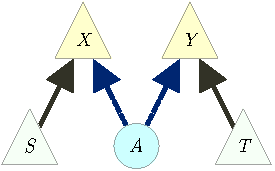
\includegraphics[width=0.7\linewidth]{BellScenarioDAG.pdf}}
\caption{(color online) The causal structure of the Bell scenario, on which Bell's theorem is based. Per convention, latent variables are indicated by circles whereas observable variables are indicated by triangles \cite{pusey2014gdag}. Observable variables with no incoming edges are setting variables, and are indicated by a light green shading.}
 \label{fig:BellDAG}
\end{figure}

Consider the causal structure associated to the Bell experiment, depicted in \cref{fig:BellDAG}. $\brackets{S,T,X,Y}$ are all observable variables whereas $A$ is the latent common cause of $X$ and $Y$.

%Without loss of generality let's assume that the values $\Lambda\mathopen{=}\lambda$ are drawn from some (possibly infinite, possibly continuous) set $\lambda\in\Omega$. 
The assumption of causal structure dictates that
\begin{align}\begin{split}\label{eq:bellstructure}
\p{x,y|s,t,a}=\p{x_s,y_t|a}=\p{x_{s|a} , y_{t|a}}
%=\p{x_{s|\lambda}}\p{y_{t|\lambda}}
\end{split}\end{align}
and accordingly that
\begin{align}\begin{split}\label{eq:bellintegration}
&\p{x_s , y_t}
=\sum\limits_{\mathclap{\lambda\in \norm{A}}}\p{x_{s|a} , y_{t|a}}\p{a}.
\end{split}\end{align}

An important causal criterion is as follows. 
\begin{prop} \label{prop:CH}
The Bell causal structure (\cref{fig:BellDAG}) implies that
\begin{align*}
%&\p{a_0 b_0} \leq \p{a_0 \nb_1} + \p{\na_1 b_0} + \p{a_1,b_1}
%\\&\text{or, letting }\;\; \p{a_0 \nb_1} \to \p{a_0}-\p{a_0 b_1}\;\text{ etc,}
%\\&\p{a_0 b_0} +\p{a_0 b_1} + \p{a_1 b_0} - \p{a_1,b_1} -\p{a_0} - \p{b_0} \leq 0
%\\&\p{x_0 , y_0} +\p{x_0 , y_1} + \p{x_1 , y_0} \leq \p{x_1 , y_1} +\p{x_0} + \p{y_0}
\p{{x}_{s^0}^{1} , {y}_{t^0}^{1}}\leq \p{\n{{x}_{s^1}^{2}} , \n{{y}_{t^1}^{2}}}+\p{{x}_{s^0}^{1} , {y}_{t^1}^{2}}+\p{{x}_{s^1}^{2} ,
   {y}_{t^0}^{1}}
\end{align*}
\end{prop}

\begin{proof}
All our proofs are based on logical tautologies, specifically tautologies of the \emph{excluded middle}. Such a tautology states that  $\NamedFunction{Or}{\alpha,\beta,\gamma,...,\,\NamedFunction{And}{\n{\alpha},\n{\beta},\n{\gamma},...,}}$. We use a variant of the tautology of the excluded middle which supplements the ``unknown" events with ``known" events, so of the form $\NamedFunction{And}{i,j}\cramp{\scriptstyle \implies}\NamedFunction{Or}{\NamedFunction{And}{\mred\alpha,j},\,\NamedFunction{And}{i,\mred\beta},\,\NamedFunction{And}{\n{\mred\alpha},\n{\mred\beta}}}$, where we have taken to highlighting the ``unknown" events in the tautology for clarity.

To prove \cref{prop:CH}, start with the \tred{latent-complete} logical tautology
\begin{align}\begin{split}
%&\parens{x_{0|\lambda} , y_{0|\lambda}} \implies\\& \parens{x_{0|\lambda} , \n{y}_{1|\lambda}} \bigvee \parens{y_{0|\lambda} , \n{x}_{1|\lambda}} \bigvee \parens*{x_{1|\lambda} , y_{1|\lambda}}.
&\hspace{-\mathindent}\NamedFunction{And}{ {x}_{s^0|a^1}^{1} , {y}_{t^0|a^1}^{1} }
 \!\!\implies \!\!
\NamedFunction{Or}{
    \NamedFunction{And}{ \n{\mred{{x}_{s^1|a^1}^{2}}} , \n{\mred{{y}_{t^1|a^1}^{2}}} } ,\\
     \NamedFunction{And}{ {x}_{s^0|a^1}^{1} , \mred{{y}_{t^1|a^1}^{2}} } ,\\
     \NamedFunction{And}{ \mred{{x}_{s^1|a^1}^{2}} , {y}_{t^0|a^1}^{1} }
}.
\end{split}\end{align}
Next, we convert the tautology to an inequality via two rules:
\begin{enumerate}
\item As the antecedent always implies the consequent, the probability of the antecedent is necessarily less-than-or-equal-to the probability of the consequent. If $j \cramp{\scriptstyle \implies} k$ then $\p{j}\leq\p{k}$.
\item The probability of a disjunction of events is less-than-or-equal-to the sum of the probabilities of the individual events, i.e. ${\p{j\lor k}=\p{j}+\p{k}-\p{j,k}\leq \p{j}+\p{k}}$.
\end{enumerate}

Thus we obtain the \tred{latent-complete} inequality
\begin{align}\begin{split}
%&p\parens{x_{0} , y_{0}|\lambda} \leq
%\\& p\parens*{\parens{x_{0} , \n{y}_{1}|\lambda} \bigvee \parens{y_{0} , \n{x}_{1}|\lambda} \bigvee \parens{x_{1} , y_{1}|\lambda}}.
&\p{{x}_{s^0|a^1}^{1} , {y}_{t^0|a^1}^{1}}\leq \p{\n{\mred{{x}_{s^1|a^1}^{2}}} , \n{\mred{{y}_{t^1|a^1}^{2}}}}\\&\qquad+\p{{x}_{s^0|a^1}^{1} ,
   \mred{{y}_{t^1|a^1}^{2}}}+\p{\mred{{x}_{s^1|a^1}^{2}} , {y}_{t^0|a^1}^{1}}.
\end{split}\end{align}

To complete the proof we simply marginalize both sides over $A$ to obtain a \tred{latent-free} inequality, which is to say we integrate over all possible values of $a$.\end{proof}

Note that we have implicitly assumed that \tred{all root vertices in the causal structure are independent}. This assumption is noteworthy, as we can apply our technique to derive inequalities for sub-DAGs, whenever the new root vertices are provably all independent. \purp{New comment, in response to Matt Pusey. Feels poorly stated. Tobias, can you find a better way of explaining where independence of settings and independence of latent variables comes into play?}

A special case of \cref{prop:CH} is obtained by choosing $x^2=\n{x^1}$. If we eliminate negation notation entirely by substituting $\p{x_{s^0} , \n{y_{t^1}}} \to \p{x_{s^0}}-\p{x_{s^0} , y_{t^1}}$ we obtain
\begin{align}\begin{split}
&\p{x_{s^0} , y_{t^0}} +\p{x_{s^0} , y_{t^1}} + \p{x_{s^1} , y_{t^0}} \\&\qquad\leq \p{x_{s^1} , y_{t^1}} +\p{x_{s^0}} + \p{y_{t^0}}
\end{split}\end{align}
which is identically the Clauser-Horne (CH) inequality \cite{CHInequality} for the Bell scenario. The CH inequality is the \emph{unique} Bell inequality (up to permutations) for the Bell scenario if $\brackets{S,T,X,Y}$ are all binary, and hence the CH inequality is a necessary and sufficient criterion to ascertain if correlations are compatible with that Bell scenario variant.


\begin{comment}
The same causal inference logic can be extended to yield polynomial inequalities. Just was we considered alternate settings values in generated out excluded middle tautology, so to we can also consider alternate values of the latent variable! For example, consider the following polynomial causal criterion.
\begin{prop} \label{prop:CHpolylite}
The Bell causal structure (\cref{fig:BellDAG}) implies that
\begin{align*}
\p{{x}_{s^0}^{1}} \p{{x}_{s^0}^{2} , {y}_{t^0}^{1}}\leq \p{\n{{y}_{t^1}^{2}}}+\p{{x}_{s^0}^{1} , {y}_{t^1}^{2}} \p{{x}_{s^0}^{2} ,
   {y}_{t^0}^{1}}
\end{align*}
\end{prop}
\begin{proof}
Start with the \tred{latent-complete} logical tautology
\begin{align}\begin{split}
&\NamedFunction{And}{ {x}_{s^0|a^2}^{1} , {x}_{s^0|a^1}^{2} , {y}_{t^0|a^1}^{1} }
 \\&\qquad\implies 
\NamedFunction{Or}{
    \n{\mred{{y}_{t^1|a^2}^{2}}} ,\\
     \NamedFunction{And}{ {x}_{s^0|a^1}^{2} , {y}_{t^0|a^1}^{1} ,\\ {x}_{s^0|a^2}^{1} , \mred{{y}_{t^1|a^2}^{2}} }
}
\end{split}\end{align}
and convert it to the \tred{latent-complete} inequality
\begin{align}\begin{split}\label{eq:chpolycond}
&\p{{x}_{s^0|a^2}^{1}} \p{{x}_{s^0|a^1}^{2} , {y}_{t^0|a^1}^{1}}\leq \p{\n{\mred{{y}_{t^1|a^2}^{2}}}}\\&\qquad+\p{{x}_{s^0|a^1}^{2} , {y}_{t^0|a^1}^{1}}
   \p{{x}_{s^0|a^2}^{1} , \mred{{y}_{t^1|a^2}^{2}}}.
\end{split}\end{align}
The factorization of the probability terms in \cref{eq:chpolycond} is allowed because \emph{any} factorization is correct. This is the benefit of dealing with deterministic events which we exploit. The particular factorization has been chosen for good reason. Note how the two instances of the latent variable are separated into distinct probabilities. This allows us to marginalize over all values of $a^1$ and then to marginalize over all values of $a^2$. Doing so concludes the proof.
\end{proof}
Many other such polynomial inequalities can be identified, see the Supplementary Materials for further examples.  
While \cref{prop:CH} is necessary and sufficient if $\brackets{S,T,X,Y}$ are all binary, polynomial generalizations such as \cref{prop:CHpolylite} may have value as novel necessary criteria for more general bipartite Bell scenarios.
\end{comment}





\section{The Triangle Scenario}

We argue that this technique for deriving polynomial inequalities for causal structures is quite general. To that end, we illustrate further detailed derivations of novel inequalities on more complex causal structure, starting with the Triangle scenario.

\begin{figure}[!t]
 \center{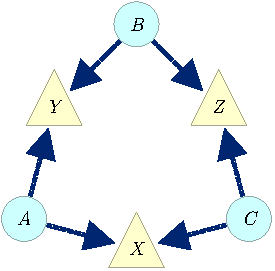
\includegraphics[width=0.7\linewidth]{TriangleScenarioDAG.pdf}}
\caption{(color online) The causal structure of the Triangle scenario, for which the three observed variables lack a common ancestor. There are no settings variables in the Triangle scenario.}
 \label{fig:TriDAG}
\end{figure}

The Triangle scenario is described by the causal structure depicted in \cref{fig:TriDAG}. Here $\brackets{X,Y,Z}$ and the observed variables, and  $\brackets{A,B,C}$ are latent. $A$ denotes the common cause of $X$ and $Y$, etc.  There can be no linear inequality in term of probabilities for the triangle scenario, which makes a polynomial inequality technique especially valuable for this scenario. The nonlinear of the Triangle scenario follows for the non-convexity of the set of all probability distributions which are compatible with it. \purp{Proof of nonconvexity or nonlinearity needed. Tobias?}

The Triangle scenario's causal structure dictates that
\begin{align}\begin{split}\label{eq:tristructure}
\p{x,y,z|a,b,c}=\p{x_{|c,a} , y_{|a,b} , z_{|b,c}}
\end{split}\end{align}
%For excessive clarity, let $\Omega_{AB}\left[\_\_\right]$ denote the complete set of values which $\lambda_{AB}$ can take, and let $\Omega_{AB}\left[a\_\right]$ denote the special subset of possible $\lambda_{AB}$ for which ${\p{a|\lambda_{AB}}\neq 0}$. %$\exists_{\lambda_{AC}}\!:\; {\p{a|\lambda_{AB}\lambda_{AC}}>0}$.
and accordingly, $\p{x,y,z}=$
\begin{align}\label{eq:triintegration}
&\hspace{-2ex}\sum\limits_{a\in \norm{A}} \sum\limits_{b\in \norm{B}} \sum\limits_{c\in \norm{C}} \p{x_{|c,a} , y_{|a,b} , z_{|b,c}}\p{a}\p{b}\p{c}.
\end{align}

Here is an example of a quadratic polynomial constraint for the Triangle scenario.
\begin{prop} \label{prop:Deg2}
The Triangle causal structure (\cref{fig:TriDAG}) implies that
\begin{align*}
&\p{{x}_{}^{1} , {y}_{}^{1} , {z}_{}^{1}} \p{{x}_{}^{2} , {y}_{}^{2} , {z}_{}^{2}}\leq \p{{y}_{}^{2}} \p{\n{{x}_{}^{3}} , \n{{z}_{}^{3}} , {y}_{}^{1}}
\\&\qquad+\p{{x}_{}^{1}} \p{{x}_{}^{2} , {z}_{}^{3}}+\p{{z}_{}^{1}} \p{{x}_{}^{3} , {z}_{}^{2}}
\end{align*}
\end{prop}
\begin{proof}
The \tred{latent-complete} tautology
\begin{align}\begin{split}
&\hspace{-\mathindent}\NamedFunction{And}{ {x}_{|c^1a^1}^{1} , {y}_{|a^1b^1}^{1} , {z}_{|b^1c^1}^{1} , {x}_{|c^2a^2}^{2} , {y}_{|a^2b^2}^{2} , {z}_{|b^2c^2}^{2}
   }
 \\&\hspace{-\mathindent}\quad\implies 
\NamedFunction{Or}{
    \NamedFunction{And}{ {y}_{|a^2b^2}^{2} , \n{\mred{{x}_{|c^2a^1}^{3}}} , \n{\mred{{z}_{|b^1c^2}^{3}}} , {y}_{|a^1b^1}^{1} } ,\\
     \NamedFunction{And}{ {x}_{|c^1a^1}^{1} , {x}_{|c^2a^2}^{2} , \mred{{z}_{|b^1c^2}^{3}} } ,\\
     \NamedFunction{And}{ {z}_{|b^1c^1}^{1} , \mred{{x}_{|c^2a^1}^{3}} , {z}_{|b^2c^2}^{2} }
}
\end{split}\end{align}
implies the \tred{latent-complete} inequality
\begin{align}\begin{split}
&\p{{x}_{|c^1a^1}^{1} , {y}_{|a^1b^1}^{1} , {z}_{|b^1c^1}^{1}} \p{{x}_{|c^2a^2}^{2} , {y}_{|a^2b^2}^{2} , {z}_{|b^2c^2}^{2}}
\\&\quad\leq \lparens{
   \p{{y}_{|a^2b^2}^{2}} \p{\n{\mred{{x}_{|c^2a^1}^{3}}} , \n{\mred{{z}_{|b^1c^2}^{3}}}
   , {y}_{|a^1b^1}^{1}}
   \\+\p{{x}_{|c^1a^1}^{1}} \p{{x}_{|c^2a^2}^{2} , \mred{{z}_{|b^1c^2}^{3}}}
   \\+\p{{z}_{|b^1c^1}^{1}} \p{\mred{{x}_{|c^2a^1}^{3}} , {z}_{|b^2c^2}^{2}}}
\end{split}\end{align}
which we can marginalize both sides over all  $\brackets{a^1,b^1,c^1,a^2,b^2,c^2}$ to obtain \cref{prop:Deg2}.
\end{proof}
Note that as a general matter, polynomial inequalities can be relaxed into interesting special cases by \emph{disregarding} some of the negated events. This type of relaxation of the polynomial inequality is related to a considering simplifications of the underlying tautology. Thus, for example, a special case of \cref{prop:Deg2} is 
\begin{align}
&\hspace{-\mathindent}\p{{y}_{}^{1} , {z}_{}^{1}} \p{ {y}_{}^{2} , {z}_{}^{2}}\leq \p{{y}_{}^{2}} \p{\n{{x}_{}^{}} , {y}_{}^{1}}+\p{{z}_{}^{1}} \p{{x}_{}^{} , {z}_{}^{2}}
\end{align}
which is plainly a consequence of the \tred{latent-complete} tautology
\begin{align}\begin{split}
&\NamedFunction{And}{ {y}_{|a^1b^1}^{1} , {z}_{|b^1c^1}^{1} , {y}_{|a^2b^2}^{2} , {z}_{|b^2c^2}^{2}
   }
 \\&\quad\implies 
\NamedFunction{Or}{
    \NamedFunction{And}{ {y}_{|a^2b^2}^{2} , \n{\mred{{x}_{|c^2a^1}^{}}} , {y}_{|a^1b^1}^{1} } ,\\
     \NamedFunction{And}{ {z}_{|b^1c^1}^{1} , \mred{{x}_{|c^2a^1}^{}} , {z}_{|b^2c^2}^{2} }
}\,.
\end{split}\end{align}



Here is an example of a cubic polynomial constraint for the Triangle scenario. 
\begin{prop} \label{prop:AllPowerful}
The Triangle causal structure (\cref{fig:TriDAG}) implies that
\begin{align*}\begin{split}
\p{{x}_{}^{1} , {y}_{}^{1} , {z}_{}^{1}}&\p{{x}_{}^{2} , {y}_{}^{2} , {z}_{}^{2}} \p{{x}_{}^{3} , {y}_{}^{3} , {z}_{}^{3}}
\\&\leq\lparens{
    \p{ \n{x^{4.\_}} , \n{y^{4.\_}} , \n{z^{4.\_}} }
\\ +\p{ {x^{1}} , {y^{4.1}} }\p{{x^{2}} }\p{ {x^{3}} , {y^{3}} , {z^{3}} }
\\ +\p{ {y^{2}} , {z^{4.1}} }\p{{y^{3}} }\p{ {x^{1}} , {y^{1}} , {z^{1}} }
\\ +\p{ {z^{3}} , {x^{4.1}} }\p{{z^{1}} }\p{ {x^{2}} , {y^{2}} , {z^{2}} }
\\ +\p{ {z^{2}} , {y^{4.2}} }\p{{z^{1}} }\p{ {x^{3}} , {y^{3}} , {z^{3}} }
\\ +\p{ {x^{3}} , {z^{4.2}} }\p{{x^{2}} }\p{ {x^{1}} , {y^{1}} , {z^{1}} }
\\ +\p{ {y^{1}} , {x^{4.2}} }\p{{y^{3}} }\p{ {x^{2}} , {y^{2}} , {z^{2}} }
   }
\end{split}\end{align*}
\end{prop}
\noindent which we will prove shortly.
In \cref{prop:AllPowerful} we have introduced the shorthand of a blank dummy index. It is a catch-all negation, such that $\n{{x}_{}^{4.\_}}=\NamedFunction{Nor}{{x}_{}^{4.1},{x}_{}^{4.2}}=\parens*{X\neq x^{4.1}\land X\neq x^{4.2}}$. Furthermore, to best leverage the inequality one should only ever use $x^{4.1}\neq x^{4.2}$. If $x$ is binary then $\brackets{x^{4.1},x^{4.2},x^{4.\_}}$ cannot be three distinct outcomes. In this case one of those three events is ``false", and any term in \cref{prop:AllPowerful} which references such an event has probability zero.
\begin{proof}\cref{prop:AllPowerful} is self-evident from the following \tred{latent-complete} inequality
\begin{align}
&\hspace{-\mathindent}\lparens{
\p{{x}_{|c^1a^1}^{1} , {y}_{|a^1b^1}^{1} , {z}_{|b^1c^1}^{1}} 
\\\times\p{{x}_{|c^2a^2}^{2} , {y}_{|a^2b^2}^{2} , {z}_{|b^2c^2}^{2}}
\\\times\p{{x}_{|c^3a^3}^{3} , {y}_{|a^3b^3}^{3} , {z}_{|b^3c^3}^{3}}}
\\\hspace{-\mathindent}&\leq\lparens{
     \p{ \n{\mred{x^{4.\_}_{|c^3 a^1}}} , \n{\mred{y^{4.\_}_{|a^1 b^2}}} , \n{\mred{z^{4.\_}_{|b^2 c^3}}} }
\\ + \p{ x^{1}_{|c^1 a^1} , \mred{y^{4.1}_{|a^1 b^2}} }\p{ x^{2}_{|a^2 c^2} }\p{ x^{3}_{|c^3 a^3} , y^{3}_{|a^3 b^3} , z^{3}_{|b^3 c^3} }
\\ + \p{ y^{2}_{|a^2 b^2} , \mred{z^{4.1}_{|b^2 c^3}} }\p{ y^{3}_{|a^3 b^3} }\p{ x^{1}_{|c^1 a^1} , y^{1}_{|a^1 b^1} , z^{1}_{|b^1 c^1} }
\\ + \p{ z^{3}_{|b^3 c^3} , \mred{x^{4.1}_{|c^3 a^1}} }\p{ z^{1}_{|b^1 c^1} }\p{ x^{2}_{|c^2 a^2} , y^{2}_{|a^2 b^2} , z^{2}_{|b^2 c^2} }
\\ + \p{ z^{2}_{|a^2 b^2} , \mred{y^{4.2}_{|a^1 b^2}} }\p{ z^{1}_{|b^1 c^1} }\p{ x^{3}_{|c^3 a^3} , y^{3}_{|a^3 b^3} , z^{3}_{|b^3 c^3} } 
\\ + \p{ x^{3}_{|c^3 a^3} , \mred{z^{4.2}_{|b^2 c^3}} }\p{ x^{2}_{|c^2 a^2} }\p{ x^{1}_{|c^1 a^1} , y^{1}_{|a^1 b^1} , z^{1}_{|b^1 c^1} } 
\\ + \p{ y^{1}_{|a^1 b^1} , \mred{x^{4.2}_{|c^3 a^1}} }\p{ y^{3}_{|a^3 b^3} }\p{ x^{2}_{|c^2 a^2} , y^{2}_{|a^2 b^2} , z^{2}_{|b^2 c^2} }
}
\nonumber\end{align}
where this time we have left out the logical tautology, as it is implicit from the \tred{latent-complete} inequality anyway.\end{proof}




A special case of \cref{prop:AllPowerful} is
\begin{prop} \label{prop:FritzF2}
The Triangle causal structure (\cref{fig:TriDAG}) implies that
\begin{align*}\begin{split}
\p{x}\p{y}\p{z}\leq& \p{\n{x},\n{y},\n{z}} + \p{x,y}\p{z} \\&\quad+ \p{y,z}\p{x} + \p{z,x}\p{y}.
\end{split}\end{align*}
\purp{strengthened!}
\end{prop}
\begin{proof}
Fist, discard all terms referencing an outcome with index ${4.2}$. Then consider the special case $x^{4.1}\to x^1$, $y^{4.1}\to y^1$, and $z^{4.1}\to z^3$. Finally, marginalize over $\brackets{y^1,z^1,x^2,z^2,x^3,y^3}$. So that only term referencing $\brackets{x^1,y^2,z^3}$ remain after marginalization.
\end{proof}


A consequence of \cref{prop:FritzF2} is that the W-type distribution
\begin{align}\label{eq:wdistribution}
p_{\text{W}}\parens{x,y,z}=\begin{cases}\tfrac{1}{3}&\text{if }\; x+y+z=1 \\ 0&\text{otherwise}\end{cases}
\end{align}
is found to be incompatible with the Triangle scenario, where $x,y,z\in\brackets{0,1}$. The W-distribution states that the in any event in which $X,Y,Z$ are observed, precisely one of them will be found to equal $1$ while the other two will equal $0$. The identity of the variable which takes the value $1$ is uniformly random. In informal but intuitive notation, the W-type distribution is ${\nicefrac{1}{3}[100]+\nicefrac{1}{3}[010]+\nicefrac{1}{3}[001]}$.
To see how this distribution is incompatible with \cref{prop:FritzF2}, note that for three \emph{identically distributed} (but not independent) binary variables a further special case of \cref{prop:FritzF2} is
\begin{align*}\begin{split}
&\hspace{-6ex}\p{X\cramp{=}1}^3\leq \p{X\cramp{=}Y\cramp{=}Z\cramp{=}0} + 3\times\p{X\cramp{=}1,Y\cramp{=}1}\p{Z\cramp{=}1}.
\end{split}\end{align*}
For the W-distribution ${\p{X\cramp{=}Y\cramp{=}Z\cramp{=}0}=0}$, and also ${\p{X\cramp{=}1,Y\cramp{=}1}=0}$, yet ${\p{X\cramp{=}1}=\nicefrac{1}{3}}$. As ${\nicefrac{1}{3^3}\nleq 0}$ we have proven that the W-type distribution is incompatible with the Triangle scenario. \purp{Original incompatibility proof was wrong, now fixed!}

%The W-distribution conflicts with Prop.~\ref{prop:TriNoGo} because ${p_{\text{W}}\parens{10\_}}={p_{\text{W}}\parens{1\_\_}}={p_{\text{W}}\parens{\_10}}={p_{\text{W}}\parens{\_1\_}}={p_{\text{W}}\parens{0\_1}}={p_{\text{W}}\parens{\_\_1}}{=\nicefrac{1}{3}}$ but ${p_{\text{W}}\parens{111}}=0$.%<\nicefrac{1}{3}$. 

\section{Failure of Entropic Inequalities}

It is interesting to note that entropic inequalities \cite{fritz2013marginal,chaves2014novel} fail to recognize the W-type distribution as incompatible with the Triangle scenario, the polynomial inequalities derivable through our method are capable of doing so. To reiterate from the abstract, enumeration of entropic inequalities is considered state-of-the-art derivation of necessary albeit insufficient causal structure compatibility criteria \cite{pusey2014gdag}. The insufficiency is a pressing concern in quantum information theory as there are uniquely-quantum distributions which cannot be certified as non-classical by means of entropic inequalities \cite{fritz2012bell}. 

%The entropic inequalities associated with the Bell scenario\footnote{Generally a non-trivial entropic inequality is defined as one that takes into account the causal structure somehow. There are no such entropic inequalities for Bell scenarios, so the inequality listed here is Shannon-type, and can be derived from nothing more than the assumption of joint measurability.} are given by
%\begin{align}\begin{split}\label{eq:entropicCHSH}
%&H\parens{A_1,B_1}+H\parens{A_0}+H\parens{B_0}
%\\&\leq H\parens{A_0,B_0}+H\parens{A_0,B_1}+H\parens{A_1,B_0}
%\end{split}\end{align}
%and its permutations \cite{chaves2014novel,chaves2012entropic}.

The entropic inequalities associated with the Triangle scenario are given by 
\begin{align}\nonumber
&I\parens{X:Y}+I\parens{X:Z}\leq H\parens{X} \\\nonumber
\text{and }\quad&I\parens{X:Y}+I\parens{X:Z}+I\parens{Y:Z}\\\label[eqs]{eq:entropicineqs}
& \leq H\parens{X,Y}-I\parens{X:Y:Z}\\\nonumber
\text{and }\quad & I\parens{X:Y}+I\parens{X:Z}+I\parens{Y:Z}\\\nonumber
& \leq\frac{H\parens{X}+H\parens{Y}+H\parens{Z}}{2}-I\parens{X:Y:Z}
\end{align}
and their permutations \cite{chaves2014novel,Chaves2015infoquantum,pusey2014gdag}.

Note that bipartite mutual information may be understood as $I\parens{X:Y}\equiv H\parens{X}+H\parens{Y}-H\parens{X,Y}$ and tripartite mutual information is defined as $I\parens{X,Y,Z}\equiv H\parens{X}+H\parens{Y}+H\parens{Z}-H\parens{X,Y}-H\parens{X,Z}-H\parens{Y,Z}+H\parens{X,Y,Z}$. It is straightforward to demonstrate that the W-type distribution given in \cref{eq:wdistribution} satisfy  \cref{eq:entropicineqs}.






\section{Deriving inequalities algorithmically}
\purp{New section, just started, to be filled in.}
We derive \tred{latent-free }polynomial inequalities by first finding \tred{latent-complete} polynomial inequalities and then marginalizing. The \tred{latent-complete} inequalities must satisfy the following requirements:

%\begin{itemize}

\noindent$\bullet$\indent Every event referenced must be deterministic without loss of generality; this is what is mean by \tred{latent-complete}. If the DAG is completed in such a manner that it permits all indeterminism to be relegated to the latent variables then a deterministic event is of one in which the observable is condition on all of its \emph{root ancestors}.

\noindent$\bullet$\indent Every event on the right hand side of the inequality but not on the left hand side should appear negated in the first term on the left hand side. Such events are the ``unkowns" in the supplemented tautology of the excluded middle. We've been highlighting them in the latent-complete inequalities presented here. We call the first term on the right hand side the ``closure" term, as it is closes the excluded middle tautology.

\noindent$\bullet$\indent Every ``uknown" event (i.e. every event on the right hand side of the inequality but not on the left hand side) should appear in precisely \emph{one} non-closure term on the left hand side. No two such events are allowed in any single term, aside from the closure term, as this would (typically) break the tautology.\footnote{Any latent-complete tautology of the form $\NamedFunction{And}{\_...}\cramp{\scriptstyle\implies}\NamedFunction{Or}{\NamedFunction{And}{\_...},\NamedFunction{And}{\_...},...}$ corresponds to a legitimate latent-complete inequality. The supplemented tautology of the excluded middle is only the easiest to construct, but others are also possible. See the proof of \cref{prop:CH}.}

\noindent$\bullet$\indent In every term, on both sides of the inequality, all instances of a latent variable with common dummy index must be restricted to the same joint probability. This is necessary in order to marginalize over the latent variables pursuant to the the causal structure. Note that unlike latent variables, a setting variable with some dummy index can appear in multiple joint probabilities in a product.

While not strictly necessary, in order to make the inequality as compelling as possible one should ensure that every event on the left hand side should also be referenced on the right hand side. If one finds an inequality lacking this property, one can tighten it by marginalizing over all such events. Such a marginalization increases the probability of the left hand side without affecting the right hand side.

Note that these polynomial inequalities are not related whatsoever to the polynomial Bell inequalities recently introduced by \citet{ChavesPolynomial} and \citet{RossetNetworks}.





\section{Other Causal Scenarios}
Here we present a few other causal structures of note and some polynomial inequalities which are justified by our method. Many more inequalities for these scenarios, and also additional scenarios, are considered in the Supplementary Materials.

\begin{figure}[t]
 \center{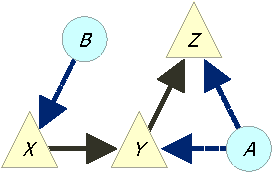
\includegraphics[width=0.7\linewidth]{InstrumentalScenarioDAG.pdf}}
\caption{(color online) The causal structure of the Instrumental scenario, which is \#1 in Ref. \cite{pusey2014gdag}. Note that we have added a second latent variable which is not usually shown for this scenario; it is required in order to relegate all indeterminism to latent variables.}
 \label{fig:InstrumentalDAG}
\end{figure}
\newpage\begin{figure}[b]
 \center{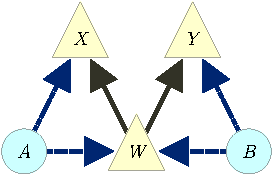
\includegraphics[width=0.7\linewidth]{EvansScenarioDAG.pdf}}
\caption{(color online) The causal structure of the Unrelated Confounding (UC) scenario \cite{evans2012graphical}, which is \#3 in Ref. \cite{pusey2014gdag}.}
 \label{fig:EvansDAG}
\end{figure}

It is also worth noting that our technique can be used to derive polynomial inequalities for subsets of the causal structure, so long as all the root vertices are independent. For example consider the truncation of the instrumental scenario show in \cref{fig:ISTruncDAG}, in which $X$ is now treated as a setting, and it, along with $A$, are the two root vertices. 

\begin{widetext}
\begin{prop}\label{prop:IS2}
The Instrumental causal structure (\cref{fig:InstrumentalDAG}) implies that
\begin{align*}
&  \p{{x}_{}^{1}} \p{{x}_{}^{3} , {y}_{}^{1} , {z}_{}^{1}}
   \leq \NamedFunction{Min}{
 \parens*{ \p{{x}_{}^{3}} \p{\n{{z}_{}^{2}} , {x}_{}^{1}}+\p{{x}_{}^{1} ,
   {z}_{}^{2}} \p{{x}_{}^{3} , {y}_{}^{1} , {z}_{}^{1}} }\,,\\\parens*{
 \p{{x}_{}^{3}} \p{\n{{y}_{}^{2}} , {x}_{}^{1}}+ \p{{x}_{}^{1} ,
   {y}_{}^{2}} \p{{x}_{}^{3} , {y}_{}^{1} , {z}_{}^{1}} }
}\,.
\\\hspace{-\mathindent}\textit{Proof:}\qquad &\p{{x}_{|b^1}^{1}} \p{{x}_{|b^2}^{3} , {y}_{|a^2b^2}^{1} , {z}_{|a^2b^2}^{1}}
   \\&\leq\NamedFunction{Min}{
 \parens*{\p{{x}_{|b^2}^{3}}  \p{\n{\mred{{z}_{|a^3b^1}^{2}}} ,
   {x}_{|b^1}^{1}}+\p{{x}_{|b^1}^{1} , \mred{{z}_{|a^3b^1}^{2}}} \p{{x}_{|b^2}^{3} ,
   {y}_{|a^2b^2}^{1} , {z}_{|a^2b^2}^{1}} }\,,\\\parens*{
 \p{{x}_{|b^2}^{3}}  \p{\n{\mred{{y}_{|a^3b^1}^{2}}} ,
   {x}_{|b^1}^{1}}+ \p{{x}_{|b^1}^{1} , \mred{{y}_{|a^3b^1}^{2}}} \p{{x}_{|b^2}^{3} ,
   {y}_{|a^2b^2}^{1} , {z}_{|a^2b^2}^{1}}}
}\,.
\end{align*}
\end{prop}
\noindent Note that \cref{prop:IS2} relies on being able to presume that $z_{|a b}$ is deterministic, even \emph{absent} knowledge of $x$ and $y$. This is an extreme application of relegating all randomness to the latent variables.




\begin{prop}
The Unrelated Confounding \cite{evans2012graphical} causal structure (\cref{fig:EvansDAG}) implies that
\begin{align*}
& \p{{w}_{}^{1} , {x}_{}^{1} , {y}_{}^{1}} \p{{w}_{}^{2} , {x}_{}^{2} , {y}_{}^{2}}
   \leq \NamedFunction{Min}{
 \parens*{\p{\n{{y}_{}^{3}}} \p{\n{{y}_{}^{4}}}+\p{{y}_{}^{4}} \p{{w}_{}^{1} , {x}_{}^{1} ,
   {y}_{}^{1}}+\p{{y}_{}^{3}} \p{{w}_{}^{2} , {x}_{}^{2} , {y}_{}^{2}} }\,,\\
 \parens*{\p{\n{{w}_{}^{3}}} \p{\n{{y}_{}^{3}}}+\p{{w}_{}^{3}} \p{{w}_{}^{1} , {x}_{}^{1} ,
   {y}_{}^{1}}+\p{{y}_{}^{3}} \p{{w}_{}^{2} , {x}_{}^{2} , {y}_{}^{2}} }\,,\\
 \parens*{\p{\n{{x}_{}^{3}}} \p{\n{{y}_{}^{3}}}+\p{{x}_{}^{3}} \p{{w}_{}^{1} , {x}_{}^{1} ,
   {y}_{}^{1}}+\p{{y}_{}^{3}} \p{{w}_{}^{2} , {x}_{}^{2} , {y}_{}^{2}} }\,,\\
 \parens*{\p{\n{{w}_{}^{3}}} \p{\n{{w}_{}^{4}}}+\p{{w}_{}^{3}} \p{{w}_{}^{1} , {x}_{}^{1} ,
   {y}_{}^{1}}+\p{{w}_{}^{4}} \p{{w}_{}^{2} , {x}_{}^{2} , {y}_{}^{2}} }
}\,.
\\\hspace{-\mathindent}\textit{Proof:}\qquad &\p{{w}_{|a^1b^1}^{1} , {x}_{|a^1b^1}^{1} , {y}_{|a^1b^1}^{1}} \p{{w}_{|a^3b^3}^{2} ,
   {x}_{|a^3b^3}^{2} , {y}_{|a^3b^3}^{2}}
   \\&\leq\NamedFunction{Min}{
 \parens*{\p{\n{\mred{{y}_{|a^2b^1}^{3}}}} \p{\n{\mred{{y}_{|a^3b^2}^{4}}}}+\p{\mred{{y}_{|a^3b^2}^{4}}}
   \p{{w}_{|a^1b^1}^{1} , {x}_{|a^1b^1}^{1} , {y}_{|a^1b^1}^{1}}+\p{\mred{{y}_{|a^2b^1}^{3}}}
   \p{{w}_{|a^3b^3}^{2} , {x}_{|a^3b^3}^{2} , {y}_{|a^3b^3}^{2}} }\,,\\
 \parens*{\p{\n{\mred{{w}_{|a^3b^2}^{3}}}} \p{\n{\mred{{y}_{|a^2b^1}^{3}}}}+\p{\mred{{w}_{|a^3b^2}^{3}}}
   \p{{w}_{|a^1b^1}^{1} , {x}_{|a^1b^1}^{1} , {y}_{|a^1b^1}^{1}}+\p{\mred{{y}_{|a^2b^1}^{3}}}
   \p{{w}_{|a^3b^3}^{2} , {x}_{|a^3b^3}^{2} , {y}_{|a^3b^3}^{2}} }\,,\\
 \parens*{\p{\n{\mred{{x}_{|a^3b^2}^{3}}}} \p{\n{\mred{{y}_{|a^2b^1}^{3}}}}+\p{\mred{{x}_{|a^3b^2}^{3}}}
   \p{{w}_{|a^1b^1}^{1} , {x}_{|a^1b^1}^{1} , {y}_{|a^1b^1}^{1}}+\p{\mred{{y}_{|a^2b^1}^{3}}}
   \p{{w}_{|a^3b^3}^{2} , {x}_{|a^3b^3}^{2} , {y}_{|a^3b^3}^{2}} }\,,\\
 \parens*{\p{\n{\mred{{w}_{|a^2b^1}^{4}}}} \p{\n{\mred{{w}_{|a^3b^2}^{3}}}}+\p{\mred{{w}_{|a^3b^2}^{3}}}
   \p{{w}_{|a^1b^1}^{1} , {x}_{|a^1b^1}^{1} , {y}_{|a^1b^1}^{1}}+\p{\mred{{w}_{|a^2b^1}^{4}}}
   \p{{w}_{|a^3b^3}^{2} , {x}_{|a^3b^3}^{2} , {y}_{|a^3b^3}^{2}} }
}\,.
\end{align*}
\end{prop}
\end{widetext}

\begin{figure}[b]
 \center{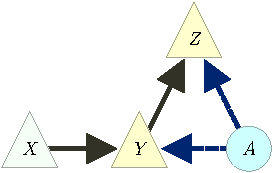
\includegraphics[width=0.7\linewidth]{TruncatedInstrumentalDAG.pdf}}
\caption{(color online) A truncation of the Instrumental scenario (\cref{fig:InstrumentalDAG}) in which $X$ is now treated as a setting.}
 \label{fig:ISTruncDAG}
\end{figure}

%It is also worth noting that our technique can be used to derive polynomial inequalities for subsets of the causal structure, so long as all the root vertices are independent. For example consider the truncation of the instrumental scenario show in \cref{fig:ISTruncDAG}, in which $X$ is now treated as a setting, and it, along with $A$, are the two root vertices. \newpage

\begin{prop}\label{prop:ISTrunc}
The truncated Instrumental causal structure (\cref{fig:ISTruncDAG}) implies that
\begin{align*}
&\hspace{-\mathindent}  \p{{y}^{1}_{x^0} , {z}^{1}_{x^0}}
   \leq \NamedFunction{Min}{
 \parens*{\p{\n{{y}^{2}_{x^1}}}+\p{{y}^{2}_{x^1}} \p{{y}^{1}_{x^0} , {z}^{1}_{x^0}}} \,,\\\parens*{
 \p{\n{{z}^{2}_{x^1}}}+\p{{z}^{2}_{x^1}} \p{{y}^{1}_{x^0} , {z}^{1}_{x^0}} }
}\,.
\\&\hspace{-\mathindent}\textit{Proof:}\qquad\p{{y}^{1}_{x^0|a^1} , {z}^{1}_{x^0|a^1}}
   \\&\leq\NamedFunction{Min}{
 \parens*{\p{\n{\mred{{y}^{2}_{x^1|a^2}}}}+\p{\mred{{y}^{2}_{x^1|a^2}}} \p{{y}^{1}_{x^0|a^1} , {z}^{1}_{x^0|a^1}} }\,,\\\parens*{
 \p{\n{\mred{{z}^{2}_{x^1|a^2}}}}+\p{\mred{{z}^{2}_{x^1|a^2}}} \p{{y}^{1}_{x^0|a^1} , {z}^{1}_{x^0|a^1}} }
}\,.
\end{align*}
\end{prop}

\begin{acknowledgments}
\bigskip\noindent\textbf{Acknowledgments}
Research at Perimeter Institute is supported by the Government of Canada through Industry Canada and by the Province of Ontario through the Ministry of Economic Development and Innovation.
\end{acknowledgments}

%\section*{References}
\nocite{*}
%\setlength{\bibsep}{\smallskipamount}
\setlength{\bibsep}{3pt plus 3pt minus 2pt}
\bibliographystyle{apsrev4-1}
%nocite{apsrev41Control}
\bibliography{apsrevcontrol,hardyinference}


\onecolumngrid
\appendix
\renewcommand{\theequation}{A-\arabic{equation}}
\setcounter{equation}{0}


%%%%%%%%%%%% Enumeration via lowercase letters
\renewcommand{\labelenumi}{(\alph{enumi})}
\renewcommand{\theenumi}{(\alph{enumi})}
\renewcommand{\labelitemi}{$\circ$}

\clearpage\section{Tobias's Original 7 Inequalities}

``I present several inequalities... together with a method of proof which has a combinatorial flavour. No quantum violations of any of these inequalities has been found to date.

In the following the complement of a value is marked by an empty circle accent, so $\mathring{b}$ means ``anything but $b$", and accordingly $P(\mathring{a}\mathring{b})=P(A\mathopen{\neq}a,B\mathopen{\neq}b)$. 
%Additionally, an underscore stands for the corresponding marginal probability, like this: $P(\_b\_) := P(abc) + P(ab\mathring{c}) + P(\mathring{a}bc) + P(\mathring{a}b\mathring{c})$. 
\begin{theorem}
The following inequalities hold for all classical correlations in the triangle scenario:
\begin{enumerate}
\item
\(\quad
%--(a)--
%P(0\_\_)P(\_\_1) \leq P(00\_)+P(\_11)
P(a) P(c)  \leq  P(a b) + P(\nb c)
\)
\item
\(\quad
%--(b)--
%P(001) P(010) P(100)  \leq  P(000) + P(11\_) P(001) P(0\_\_) + P(1\_1) P(010) P(\_\_0) + P(\_11) P(100) P(\_0\_)
P(a b\nc) P(a \nb c) P(\na b c) \leq P(a b c) + P(\na \nb) P(a b \nc) P(a) + P(\na\nc) P(a\nb c) P(c)  + P(\nb \nc) P(\na b c) P(b)
\)
\item 
\(\quad
%--(c)--
%P(001) P(010) P(100) \leq  P(000)^2 + 2 P(11\_) P(001) + 2 P(1\_1) P(010) + 2 P(\_11) P(100)
P(a b\nc) P(a \nb c) P(\na b c) \leq P(a b c)^2 + 2\parens*{P(\na \nb) P(a b \nc) + P(\na\nc) P(a\nb c)  + P(\nb \nc) P(\na b c)}
\)
\item
\(\quad
%--(d)--
%P(000)^2 P(111)  \leq  P(001) P(010) P(100) + (2 P(000) + P(111)) (1 - P(000) - P(111))
P(a b c)^2 P(\na\nb\nc)  \leq  P(a b \nc) P(a \nb c) P(\na b c) + \parens*{2 P(a b c) + P(\na\nb\nc)} \parens*{1 - P(a b c) - P(\na\nb\nc)}
\)
\item
\(\quad
%--(e)--
%P(000)^2 P(111)  \leq  P(000)^3 + (2 P(000) + P(111)) (1 - P(000) - P(111))
P(a b c)^2 P(\na\nb\nc)  \leq  P(a b c)^3 + \parens*{2 P(a b c) + P(\na\nb\nc)} \parens*{1 - P(a b c) - P(\na\nb\nc)}
\)
\item
\(\quad
%--(f)--
%P(1\_\_)P(\_1\_)P(\_\_1) \leq P(000)+P(11\_)P(\_\_1)+P(1\_1)P(\_1\_)+P(\_11)P(1\_\_)
P(a) P(b) P(c) \leq  P(\na\nb\nc) + P(a b) P(c) + P(a c) P(b) + P(b c) P(a)
\)
\item
\(\quad
%--(g)--
%P(1\_\_)P(\_1\_)P(\_\_1) \leq P(000)^2+2 P(11\_)P(\_\_1) + 2 P(1\_1)P(\_1\_) + 2 P(\_11)P(1\_\_)
P(a) P(b) P(c) \leq  P(\na\nb\nc)^2 +2\parens[\Big]{ P(a b) P(c) + P(a c) P(b) + P(b c) P(a) }
\)
\end{enumerate}
\end{theorem}

It is quite likely that some of these inequalities are dominated by the others, but I do not know for sure whether any of them are actually redundant."

\purp{Note that \cref{prop:AllPowerful} implies inequalities (a), (b), and (f), BUT NOT THE OTHERS, as the others involve \emph{independent} negation closures.\\
\indent Happily, the other inequalities are implied by additional cubic inequalities generated by the Mathematica code.
}

\begin{comment}
\section{Copy and Paste Playground}
\begin{align}
\parens{
    {x}_{s^0}^{\lambda ^2} , {x}_{s^0}^{\lambda ^1} , {y}_{t^0}^{\lambda ^1}
}
&\implies 
\NamedFunction{Or}{
    \n{{y}_{t^1}^{\lambda ^2}} ,\\
     \parens{
        {x}_{s^0}^{\lambda ^1} , {y}_{t^0}^{\lambda ^1} , {x}_{s^0}^{\lambda ^2} , {y}_{t^1}^{\lambda ^2}
    }
} \\
\parens{
    {x}_{s^0}^{\lambda ^1} , {y}_{t^0}^{\lambda ^1} , {x}_{s^0}^{\lambda ^2} , {y}_{t^0}^{\lambda ^2}
}
&\implies 
\NamedFunction{Or}{
    \parens{
        \n{{x}_{s^1}^{\lambda ^2}} , \n{{y}_{t^1}^{\lambda ^1}}
    } ,\\
     \parens{
        {x}_{s^0}^{\lambda ^2} , {x}_{s^0}^{\lambda ^1} , {y}_{t^1}^{\lambda ^1}
    } ,\\
     \parens{
        {x}_{s^0}^{\lambda ^1} , {y}_{t^0}^{\lambda ^1} , {x}_{s^1}^{\lambda ^2} , {y}_{t^0}^{\lambda ^2}
    }
}\\
\parens{
    {x}_{s^0}^{\lambda ^1} , {y}_{t^0}^{\lambda ^1} , {x}_{s^0}^{\lambda ^2} , {y}_{t^0}^{\lambda ^2}
}
&\implies 
\NamedFunction{Or}{
    \parens{
        \n{{x}_{s^1}^{\lambda ^2}} , \n{{y}_{t^1}^{\lambda ^2}}
    } ,\\
     \parens{
        {x}_{s^0}^{\lambda ^1} , {y}_{t^0}^{\lambda ^1} , {x}_{s^0}^{\lambda ^2} , {y}_{t^1}^{\lambda ^2}
    } ,\\
     \parens{
        {x}_{s^0}^{\lambda ^1} , {y}_{t^0}^{\lambda ^1} , {x}_{s^1}^{\lambda ^2} , {y}_{t^0}^{\lambda ^2}
    }
}
\end{align}
\end{comment}
\end{document}